\documentclass[12pt,a4paper]{article}
\usepackage{ctex}
\usepackage{geometry}
\usepackage{amsmath,amssymb}
\usepackage{graphicx}
\usepackage{listings}
\usepackage{xcolor}
\usepackage{multirow}
\graphicspath{{../chp3/figs/}}

% 定义颜色
\definecolor{codegreen}{rgb}{0,0.6,0}
\definecolor{codegray}{rgb}{0.5,0.5,0.5}
\definecolor{codepurple}{rgb}{0.58,0,0.82}
\definecolor{backcolour}{rgb}{0.95,0.95,0.92}

\lstset{
  language=Python,
  basicstyle=\ttfamily\small,
  backgroundcolor=\color{backcolour},   % 背景颜色
  commentstyle=\color{codegreen},       % 注释颜色
  keywordstyle=\color{magenta},         % 关键字颜色
  numberstyle=\tiny\color{codegray},    % 行号颜色
  stringstyle=\color{codepurple},       % 字符串颜色
  frame=single,                         % 在代码周围画框
  rulecolor=\color{black},              % 框颜色
  breaklines=true,
  columns=fullflexible,
  showstringspaces=false,
  numbers=left,                         % 显示行号
  numbersep=5pt,                        % 行号间距
  tabsize=2,                            % tab大小
  captionpos=b                          % 标题位置
}
\geometry{left=2.5cm,right=2.5cm,top=2.5cm,bottom=2.5cm}

\title{高等工程热力学\\第3章作业}
\author{姓名:\underline{\hspace{4cm}} \quad 学号:\underline{\hspace{4cm}}}
\date{\today}

\begin{document}
\renewcommand{\maketitle}{}
\maketitle

\section*{第三章}

\subsection*{3-10}
采用Python语言进行计算程序编写,计算思路如下:

(1)导入参数临界温度$T_\mathrm{c}$、临界压力$p_\mathrm{c}$、偏心因子$\omega$、摩尔质量$M$和理想气体常数$R=8.314462618\mathrm{J/(mol\cdot K)}$;

(2)给定温度$T$计算参数$a$和$b$;

(3)给定温度$T$和压力$p$计算参数$A$和$B$;

(4)计算压缩因子$Z$的多项式系数$C_2, C_1, C_0$;

(5)使用牛顿法分别计算压缩因子$Z$的液相值$Z_l$和气相值$Z_g$;

(6)计算比体积$v$的液相值$v_l$和气相值$v_g$;

(7)在给定压力$p$下,绘制比体积$v$与温度$T$的关系曲线,并标注饱和温度$T_\mathrm{sat}$。

计算程序如下:
\begin{lstlisting}
import numpy as np
import matplotlib.pyplot as plt
import os

# 使用 Times New Roman 作为 matplotlib 全局字体
plt.rcParams["font.family"] = "serif"
plt.rcParams["font.serif"] = ["Times New Roman"]
plt.rcParams["mathtext.fontset"] = "stix"


class PRFluid:
    def __init__(self, Tc, Pc, omega, M):
        self.Tc = Tc  # 输入K
        self.Pc = Pc * 1e6  # 输入MPa
        self.omega = omega  # 无量纲
        self.M = M / 1000  # 输入g/mol

    R = 8.314462618  # J/(mol*K)

    # 计算a和b
    def params(self, T):
        kappa = 0.37464 + 1.54226 * self.omega - 0.26992 * self.omega**2
        Tr = T / self.Tc
        alpha = (1 + kappa * (1 - Tr**0.5)) ** 2
        a = 0.45724 * self.R**2 * self.Tc**2 / self.Pc * alpha
        b = 0.07780 * self.R * self.Tc / self.Pc
        return a, b

    # 计算A和B
    def AB(self, T, p):
        a, b = self.params(T)
        A = a * p * 1e6 / (self.R * T) ** 2
        B = b * p * 1e6 / (self.R * T)
        return A, B

    # 计算C2, C1, C0
    def C(self, T, p):
        A, B = self.AB(T, p)
        C2 = -(1 - B)
        C1 = A - 3 * B**2 - 2 * B
        C0 = -(A * B - B**2 - B**3)
        return C2, C1, C0

    # 计算压缩因子Z
    # 液相
    def Zl(self, T, p):
        C2, C1, C0 = self.C(T, p)
        # 牛顿法求解Z
        Zl = 0.001  # 初始猜测值
        for _ in range(100):
            f = Zl**3 + C2 * Zl**2 + C1 * Zl + C0
            df = 3 * Zl**2 + 2 * C2 * Zl + C1
            Zl_new = Zl - f / df
            if abs(Zl_new - Zl) < 1e-6:
                break
            Zl = Zl_new
        return Zl

    # 气相
    def Zg(self, T, p):
        C2, C1, C0 = self.C(T, p)
        # 牛顿法求解Z
        Zg = 1.0  # 初始猜测值
        for _ in range(100):
            f = Zg**3 + C2 * Zg**2 + C1 * Zg + C0
            df = 3 * Zg**2 + 2 * C2 * Zg + C1
            Zg_new = Zg - f / df
            if abs(Zg_new - Zg) < 1e-6:
                break
            Zg = Zg_new
        return Zg

    # 计算比体积v
    # 液相
    def vl(self, T, p):
        Zl = self.Zl(T, p)
        vl = Zl * self.R * T / (p * 1e6 * self.M)
        return vl

    # 气相
    def vg(self, T, p):
        Zg = self.Zg(T, p)
        vg = Zg * self.R * T / (p * 1e6 * self.M)
        return vg

    # 画v-T图
    def plot_Tv(
        self,
        fluid_name,  # 流体名称
        p,  # 压力 Pa
        Tsat,  # 饱和温度 K
        T_min,  # 温度范围最小值 K
        T_max,  # 温度范围最大值 K
        nT=220,  # 温度点数
    ):
        T_grid = np.linspace(T_min, T_max, nT)  # 温度网格
        v_grid = np.empty_like(T_grid)  # 比体积网格
        # 计算比体积
        for i, T in enumerate(T_grid):
            if T < Tsat:
                v_grid[i] = self.vl(T, p)
            elif T > Tsat:
                v_grid[i] = self.vg(T, p)
            else:
                v_grid[i] = 0.5 * (self.vl(T, p) + self.vg(T, p))
        fig, ax = plt.subplots()  # 创建图像和坐标轴
        # 主曲线
        ax.plot(v_grid, T_grid, linewidth=2, label=fluid_name)
        xmin, xmax = np.nanmin(v_grid), np.nanmax(v_grid)
        # Tsat 虚线
        ax.hlines(Tsat, xmin, xmax, linestyles="--", label=r"$T_{\mathrm{sat}}$")
        # 标注 Tsat
        yt = list(ax.get_yticks())
        # 加入Tsat并排序
        if not any(abs(t - Tsat) < 1e-8 for t in yt):
            yt.append(Tsat)
        yt = np.array(sorted(yt))
        # 生成刻度标签:对 Tsat 使用仅数值标签(两位小数),其它刻度保留数字格式(根据范围选择小数位)
        deltaT = T_grid.max() - T_grid.min()
        labels = []
        for t in yt:
            if abs(t - Tsat) < 1e-8 or abs(t - Tsat) < 1e-6 * max(1.0, deltaT):
                labels.append(f"{Tsat:.2f}")
            else:
                # 根据温度范围决定格式,避免过多小数
                if deltaT > 50:
                    labels.append(f"{t:.0f}")
                else:
                    labels.append(f"{t:.2f}")
        ax.set_yticks(yt)
        ax.set_yticklabels(labels)
        # 轴标签
        ax.set_xlabel(r"$v$ (m³/kg)")
        ax.set_ylabel(r"$T$ (K)")
        # 标题
        ax.set_title(f"{fluid_name}  $v$–$T$ at $p$ = {p:.1f} MPa")
        ax.grid(True)
        ax.set_xscale("log")  # 使用对数刻度
        ax.legend(loc="upper left", frameon=True, fancybox=True, framealpha=0.9)

        # 固定保存路径为脚本同目录下的 figs 文件夹
        base_dir = os.path.dirname(os.path.abspath(__file__))
        fig_dir = os.path.join(base_dir, "figs")
        os.makedirs(fig_dir, exist_ok=True)

        # 文件名固定为"流体名称.png"
        filename = f"{fluid_name}.png"
        savepath = os.path.join(fig_dir, filename)

        # 保存图像,固定参数
        fig.savefig(savepath, dpi=300, bbox_inches="tight", transparent=False)
        plt.close(fig)


# 实际计算
R290 = PRFluid(369.89, 4.2512, 0.1521, 44.096)
R290.plot_Tv("R290", 1.4, 317.86, 200, 450)

R600a = PRFluid(407.81, 3.629, 0.184, 58.122)
R600a.plot_Tv("R600a", 0.6, 314.12, 200, 450)

\end{lstlisting}

R290在1.4MPa下的$T$-$v$图和R600a在0.6MPa下的$T$-$v$图如下:
\begin{figure}[ht]
    \centering
    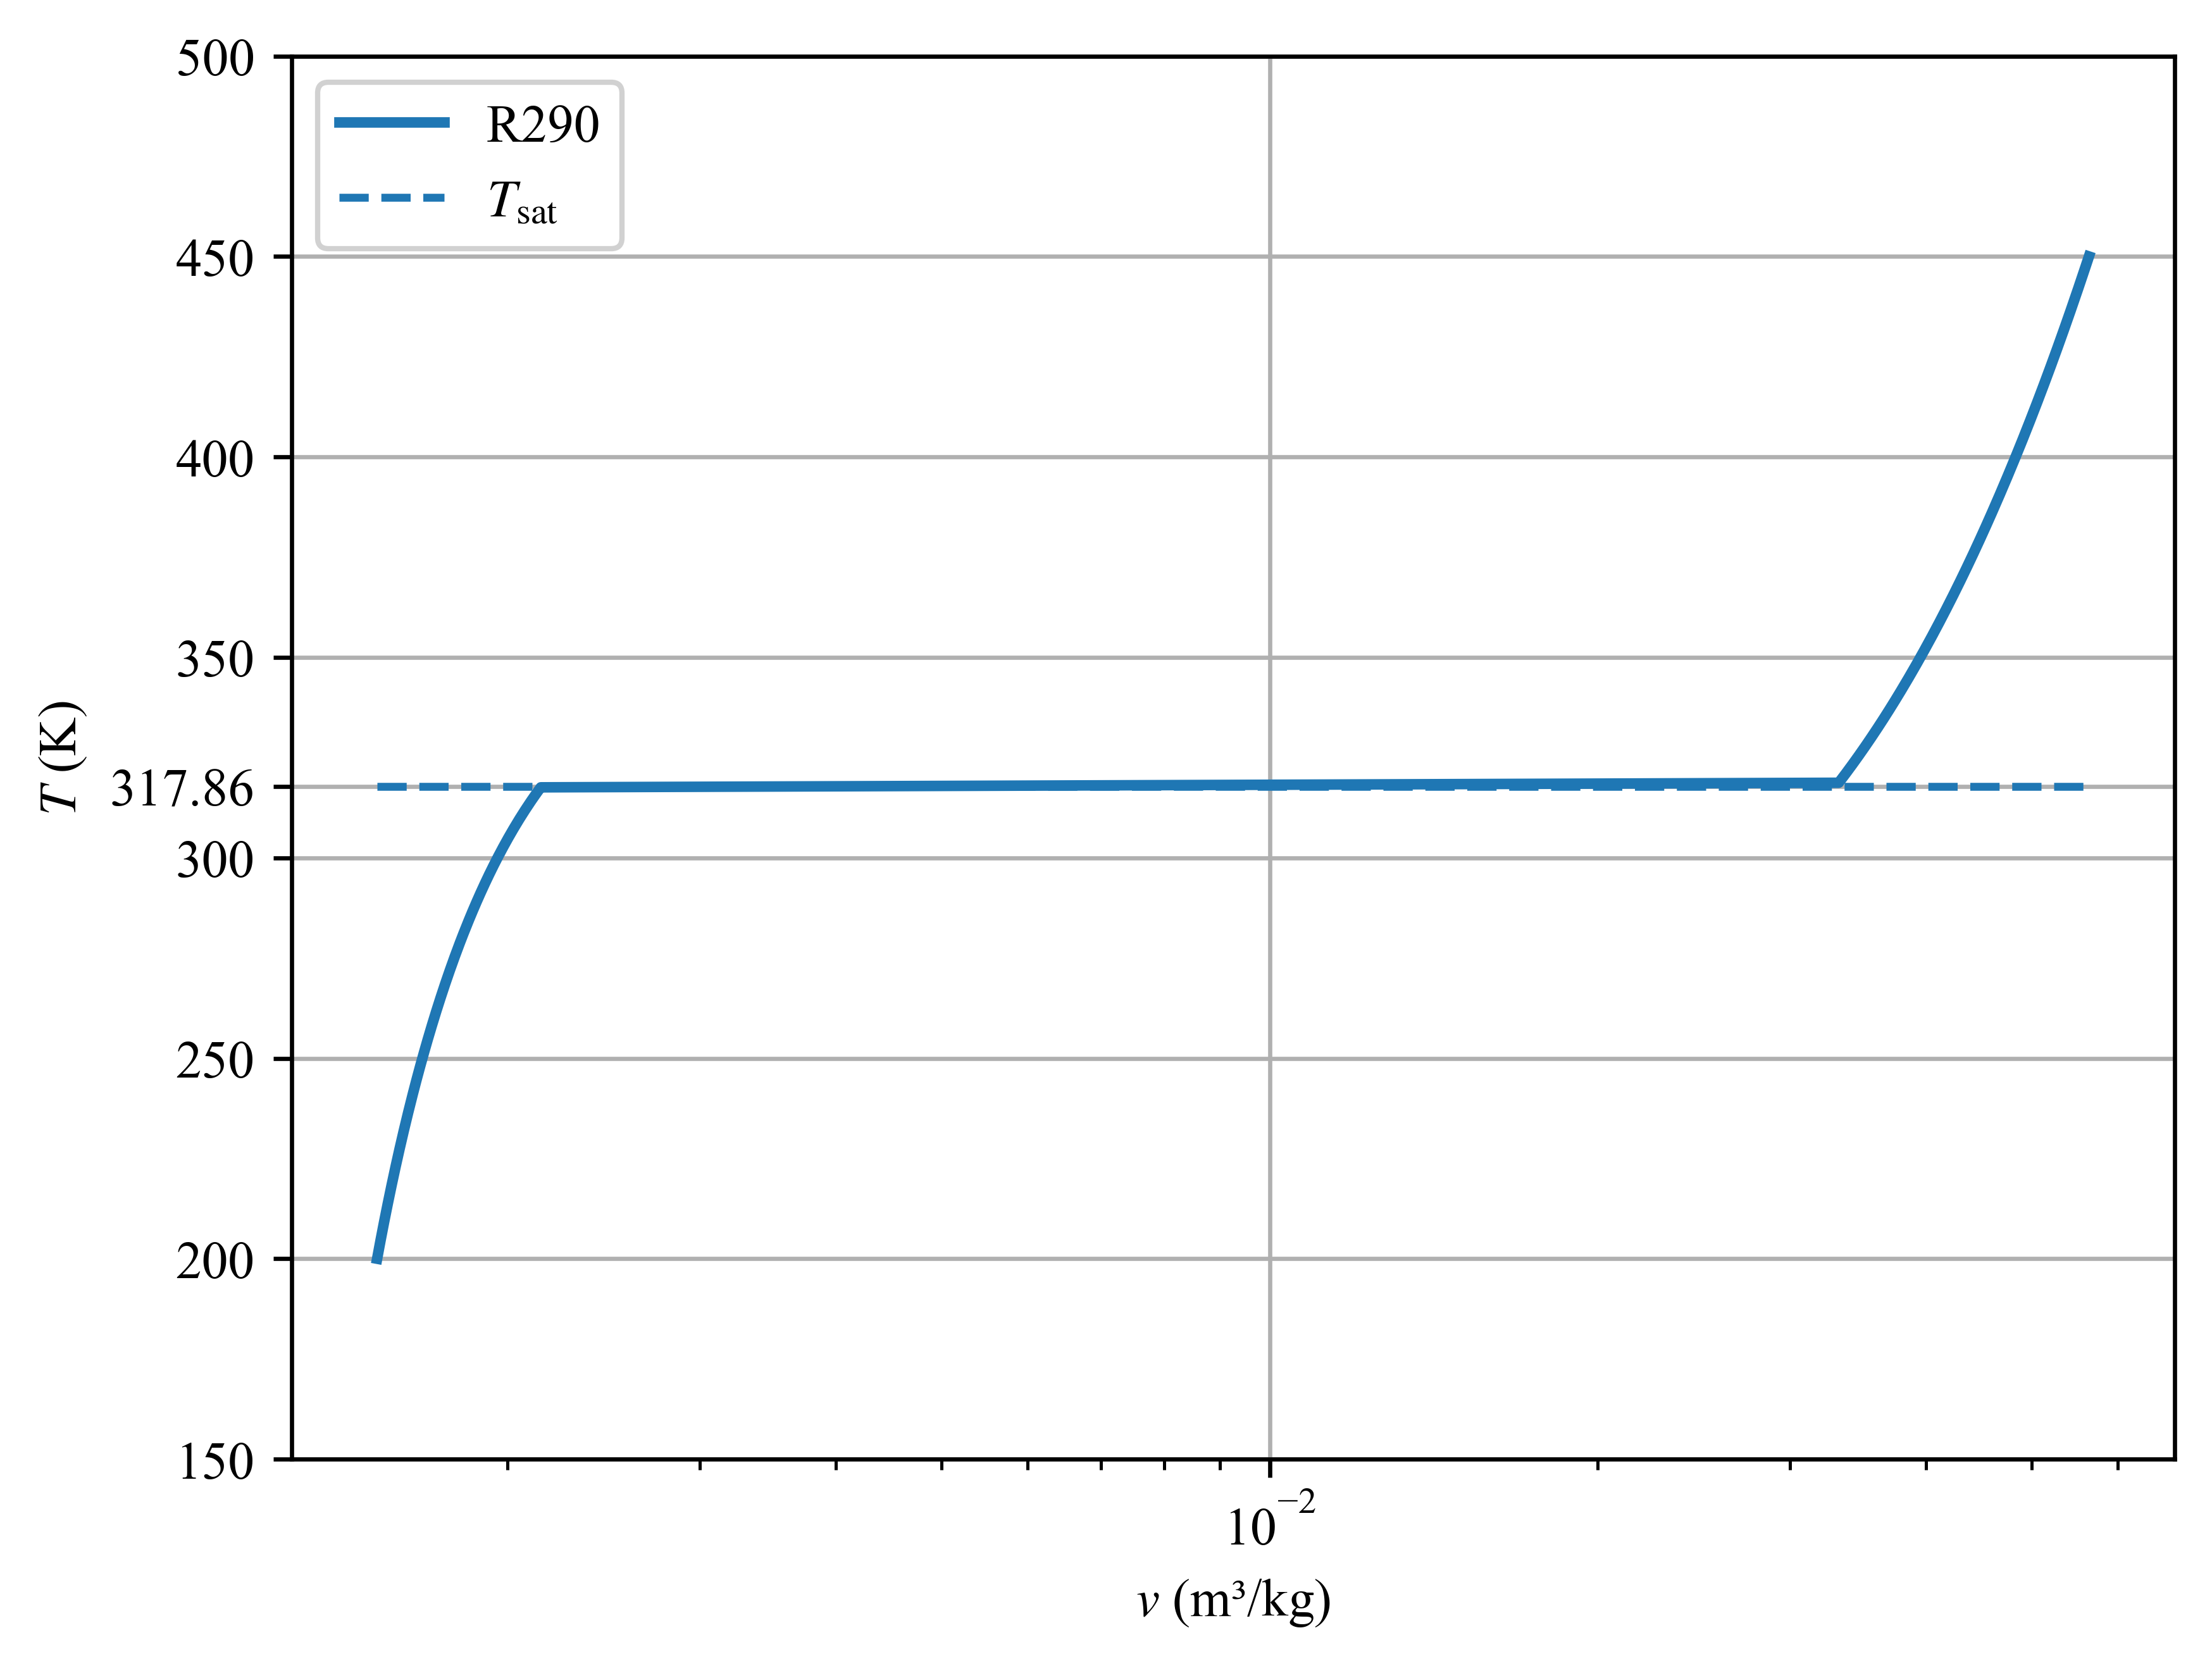
\includegraphics[width=0.7\textwidth]{R290.png}
    \caption{R290在1.4MPa下的$T$-$v$图}
\end{figure}

\begin{figure}[ht]
    \centering
    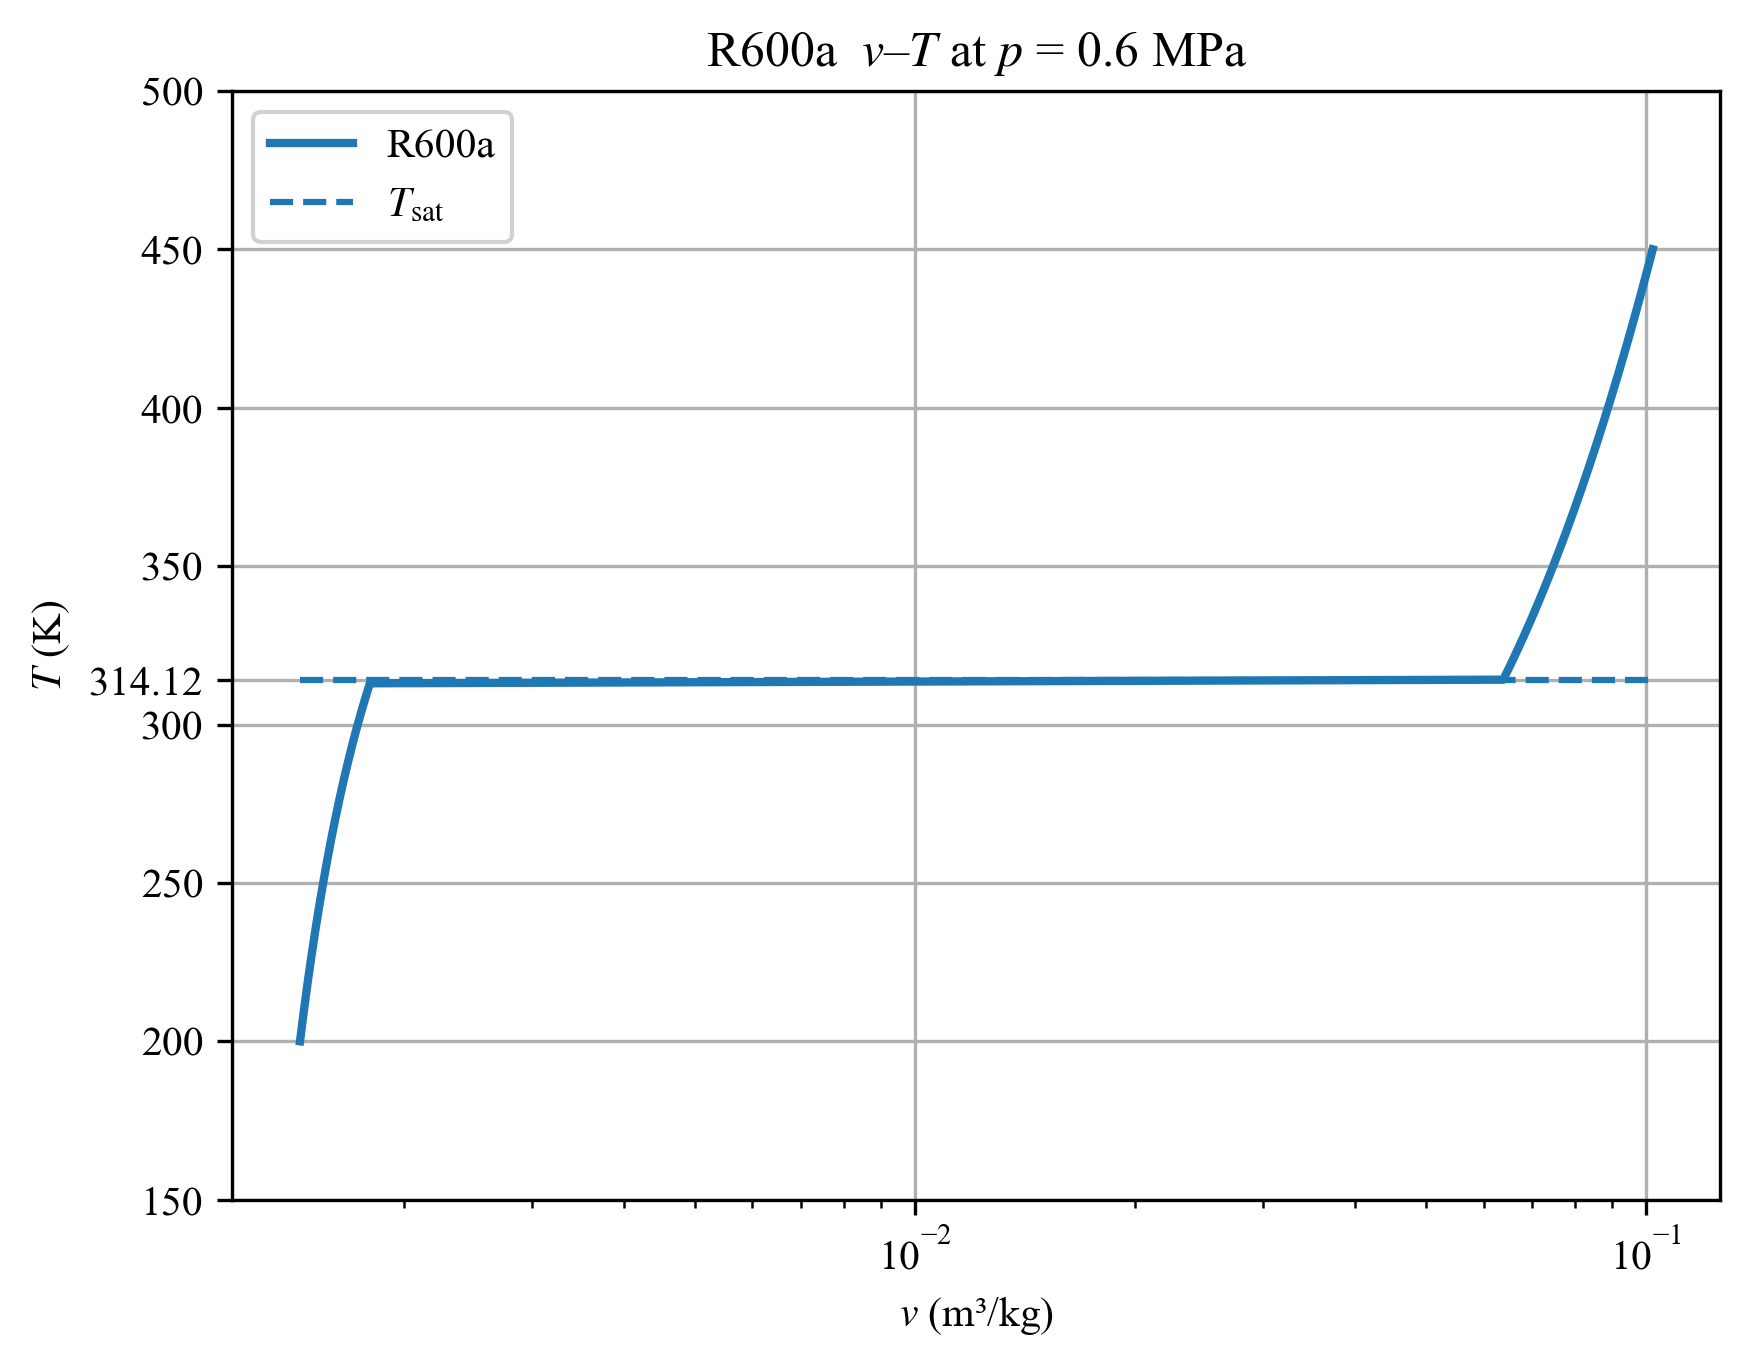
\includegraphics[width=0.7\textwidth]{R600a.png}
    \caption{R600a在0.6MPa下的$T$-$v$图}
\end{figure}

\subsection*{3-13}
查物性库得,对于R134a,各参数为:$T_\mathrm{c}=374.21\mathrm{K}$,$p_\mathrm{c}=4.0593\mathrm{MPa}$,$\omega=0.326$,$M=102.03\mathrm{g/mol}$。

对于R1234yf,各参数为:$T_\mathrm{c}=367.85\mathrm{K}$,$p_\mathrm{c}=3.3822\mathrm{MPa}$,$\omega=0.276$,$M=114.04\mathrm{g/mol}$;

对于R1234ze(E),各参数为:$T_\mathrm{c}=382.75\mathrm{K}$,$p_\mathrm{c}=3.6349\mathrm{MPa}$,$\omega=0.313$,$M=114.04\mathrm{g/mol}$;

压力为0.1MPa,温度为35℃=308.15K时,以上三种制冷剂均为气相。利用题3-10程序进行计算$v_g$,计算结果为:

$v_\mathrm{R134a}=0.24679\mathrm{m^3/kg}$,$v_\mathrm{R1234yf}=0.22031\mathrm{m^3/kg}$,$v_\mathrm{R1234ze(E)}=0.22007\mathrm{m^3/kg}$

可以看出,三种制冷剂的比体积相差不大,R134a的比体积略大于另外两种。

\subsection*{3-15}
在题3-10的程序基础上,更改\_\_init\_\_函数与a、b计算函数params,更改如下:
\begin{lstlisting}
class FRFluid2:
    def __init__(self, Tc1, Tc2, pc1, pc2, omega1, omega2, M1, M2, x1, kij):
        self.Tc1 = Tc1  # K
        self.Tc2 = Tc2  # K
        self.pc1 = pc1 * 1e6  # Pa,输入MPa,改为乘法
        self.pc2 = pc2 * 1e6  # Pa,输入MPa,改为乘法
        self.omega1 = omega1  # 无量纲
        self.omega2 = omega2  # 无量纲
        self.M1 = M1 / 1e3  # kg/mol,输入g/mol
        self.M2 = M2 / 1e3  # kg/mol,输入g/mol
        self.x1 = x1  # 组分1的摩尔分率
        self.x2 = 1 - x1  # 组分2的摩尔分率
        self.kij = kij  # 组分间的二元交互作用参数

    R = 8.314462618  # J/(mol*K)

    # 计算a和b
    def params(self, T):
        kappa1 = 0.37464 + 1.54226 * self.omega1 - 0.26992 * self.omega1**2
        kappa2 = 0.37464 + 1.54226 * self.omega2 - 0.26992 * self.omega2**2
        Tr1 = T / self.Tc1
        Tr2 = T / self.Tc2
        alpha1 = (1 + kappa1 * (1 - Tr1**0.5)) ** 2
        alpha2 = (1 + kappa2 * (1 - Tr2**0.5)) ** 2
        a1 = 0.45724 * self.R**2 * self.Tc1**2 / self.pc1 * alpha1
        a2 = 0.45724 * self.R**2 * self.Tc2**2 / self.pc2 * alpha2
        b1 = 0.07780 * self.R * self.Tc1 / self.pc1
        b2 = 0.07780 * self.R * self.Tc2 / self.pc2
        a = (
            self.x1**2 * a1
            + self.x2**2 * a2
            + 2 * self.x1 * self.x2 * (a1 * a2) ** 0.5 * (1 - self.kij)
        )
        b = self.x1 * b1 + self.x2 * b2
        return a, b

\end{lstlisting}

在压力$p=0.1\mathrm{MPa}$、$0.2\mathrm{MPa}$、$0.3\mathrm{MPa}$,温度$T=300\mathrm{K}$时,不同的$k_{ij}$条件下,混合制冷剂R290/R600a的比体积计算结果与计算偏差如表1所示,表中计算偏差是相对于$k_{ij}=0.064$时的比体积计算结果而言的。可以看出,$k_{ij}$取0.1、0和-0.1时,计算结果与$k_{ij}=0.064$时的比体积计算结果偏差逐渐增大,且偏差均小于1\%。
\begin{table}[h]
\centering
\begin{tabular}{c c c c}
\hline
$p$ (MPa) & $k_{ij}$ &  $v$ (m³/kg) &误差 (\%) \\
\hline
\multirow{4}{*}{0.1} & 0.064 & 0.47838 &   \\
 & 0.1 & 0.47859 & 0.04390\\
 & 0 & 0.47802 & 0.07525  \\
 & -0.1 & 0.47744 & 0.19650  \\
\hline
\multirow{4}{*}{0.2} & 0.064 & 0.23422 &   \\
 & 0.1 & 0.23443 & 0.08966  \\
 & 0 & 0.23384 & 0.16224  \\
 & -0.1 & 0.23324 & 0.41841  \\
\hline
\multirow{4}{*}{0.3} & 0.064 & 0.15273 &   \\
 & 0.1 & 0.15295 & 0.14405  \\
 & 0 & 0.15233 & 0.26190  \\
 & -0.1 & 0.15171 & 0.66785  \\
\hline
\end{tabular}
\caption{不同$k_{ij}$条件下混合制冷剂R290/R600a的比体积计算结果与计算偏差}

\end{table}

\newpage

\section*{第四章}

\subsection*{4-13}

在题3-10程序的基础上扩充,采用Python语言进行计算程序编写,计算程序如下:

\begin{lstlisting}
# 理清各压力单位,三个压力,临界压力pc,0℃的饱和压力ps0,计算时的压力p
import numpy as np


class PRHS:
    def __init__(self, Tc, pc, omega, M, ps0):
        self.Tc = Tc  # K
        self.pc = pc * 1e6  # Pa,输入MPa
        self.omega = omega  # 无量纲
        self.M = M / 1e3  # kg/mol,输入g/mol
        self.ps0 = ps0  # MPa

    R = 8.314462618  # J/(mol*K)

    # 计算a和b
    def params(self, T):
        kappa = 0.37464 + 1.54226 * self.omega - 0.26992 * self.omega**2
        Tr = T / self.Tc
        alpha = (1 + kappa * (1 - Tr**0.5)) ** 2
        a = 0.45724 * self.R**2 * self.Tc**2 / self.pc * alpha
        da = (
            -0.45724
            * self.R**2
            * self.Tc**2
            / self.pc
            * kappa
            * (1 + kappa * (1 - Tr**0.5))
            * (Tr**-0.5)
            / self.Tc
        )
        b = 0.07780 * self.R * self.Tc / self.pc
        return a, b, da

    # 计算A和B
    def AB(self, T, p):
        a, b, da = self.params(T)
        A = a * p * 1e6 / (self.R * T) ** 2  # p从MPa转换为Pa
        B = b * p * 1e6 / (self.R * T)  # p从MPa转换为Pa
        return A, B

    # 计算C2, C1, C0
    def C(self, T, p):
        A, B = self.AB(T, p)
        C2 = -(1 - B)
        C1 = A - 3 * B**2 - 2 * B
        C0 = -(A * B - B**2 - B**3)
        return C2, C1, C0

    # 计算压缩因子Z
    # 液相
    def Zl(self, T, p):
        C2, C1, C0 = self.C(T, p)
        # 牛顿法求解Z
        Zl = 0.001  # 初始猜测值
        for _ in range(100):
            f = Zl**3 + C2 * Zl**2 + C1 * Zl + C0
            df = 3 * Zl**2 + 2 * C2 * Zl + C1
            Zl_new = Zl - f / df
            if abs(Zl_new - Zl) < 1e-6:
                break
            Zl = Zl_new
        return Zl

    # 气相
    def Zg(self, T, p):
        C2, C1, C0 = self.C(T, p)
        # 牛顿法求解Z
        Zg = 1.0  # 初始猜测值
        for _ in range(100):
            f = Zg**3 + C2 * Zg**2 + C1 * Zg + C0
            df = 3 * Zg**2 + 2 * C2 * Zg + C1
            Zg_new = Zg - f / df
            if abs(Zg_new - Zg) < 1e-6:
                break
            Zg = Zg_new
        return Zg

    # 计算比体积v
    # 液相
    def vl(self, T, p):
        Zl = self.Zl(T, p)
        vl = Zl * self.R * T / (p * 1e6)  # p从MPa转换为Pa
        return vl

    # 气相
    def vg(self, T, p):
        Zg = self.Zg(T, p)
        vg = Zg * self.R * T / (p * 1e6)  # p从MPa转换为Pa
        return vg

    # 计算焓的余函数
    # 液相
    def h_res_l(self, T, p):
        a, b, da = self.params(T)
        Zl = self.Zl(T, p)
        vl = self.vl(T, p)
        hr_l = (T * da - a) / (b * np.sqrt(8)) * np.log(
            (vl - 0.414 * b) / (vl + 2.414 * b)
        ) + self.R * T * (1 - Zl)
        return hr_l

    # 气相
    def h_res_g(self, T, p):
        a, b, da = self.params(T)
        Zg = self.Zg(T, p)
        vg = self.vg(T, p)
        hr_g = (T * da - a) / (b * np.sqrt(8)) * np.log(
            (vg - 0.414 * b) / (vg + 2.414 * b)
        ) + self.R * T * (1 - Zg)
        return hr_g

    # 计算熵的余函数
    # 液相
    def s_res_l(self, T, p):
        a, b, da = self.params(T)
        vl = self.vl(T, p)
        sr_l = (
            -self.R * np.log((vl - b) / vl)
            - self.R * np.log(vl / (self.R * T / (p * 1e6)))
            + da / (b * np.sqrt(8)) * np.log((vl - 0.414 * b) / (vl + 2.414 * b))
        )
        return sr_l

    # 气相
    def s_res_g(self, T, p):
        a, b, da = self.params(T)
        vg = self.vg(T, p)
        sr_g = (
            -self.R * np.log((vg - b) / vg)
            - self.R * np.log(vg / (self.R * T / (p * 1e6)))
            + da / (b * np.sqrt(8)) * np.log((vg - 0.414 * b) / (vg + 2.414 * b))
        )
        return sr_g

    # 计算c_p积分
    def cp(self, T, A, B, C, D):
        cp = (
            A * (T - 273.15)
            + B / 2 * (T**2 - 273.15**2)
            + C / 3 * (T**3 - 273.15**3)
            + D / 4 * (T**4 - 273.15**4)
        )
        return cp

    # 计算c_p/T积分
    def cpT(self, T, A, B, C, D):
        cp = (
            A * np.log(T / 273.15)
            + B * (T - 273.15)
            + C / 2 * (T**2 - 273.15**2)
            + D / 3 * (T**3 - 273.15**3)
        )
        return cp

    # 计算焓和熵
    # 液相
    def h_l(self, T, A, B, C, D, p):
        h_r_ps_0 = self.h_res_l(273.15, self.ps0)
        cp0 = self.cp(T, A, B, C, D)
        h_res_l = self.h_res_l(T, p)
        hl = 200 * 1e3 + cp0 + (h_r_ps_0 - h_res_l) / self.M  # J/kg
        return hl

    def s_l(self, T, A, B, C, D, p):
        s_r_ps_0 = self.s_res_l(273.15, self.ps0)
        cpT = self.cpT(T, A, B, C, D)
        sr_l = self.s_res_l(T, p)
        sl = (
            1e3 + cpT + (s_r_ps_0 - self.R * np.log(p / self.ps0) - sr_l) / self.M
        )  # J/(kg*K)
        return sl

    # 气相
    def h_g(self, T, A, B, C, D, p):
        h_r_ps_0 = self.h_res_l(273.15, self.ps0)  # 使用液相作为基准
        cp0 = self.cp(T, A, B, C, D)
        h_res_g = self.h_res_g(T, p)
        hg = 200 * 1e3 + cp0 + (h_r_ps_0 - h_res_g) / self.M  # J/kg
        return hg

    def s_g(self, T, A, B, C, D, p):
        s_r_ps_0 = self.s_res_l(273.15, self.ps0)  # 使用液相作为基准
        cpT = self.cpT(T, A, B, C, D)
        sr_g = self.s_res_g(T, p)
        sg = (
            1e3 + cpT + (s_r_ps_0 - self.R * np.log(p / self.ps0) - sr_g) / self.M
        )  # J/(kg*K)
        return sg


R290 = PRHS(369.89, 4.2512, 0.1521, 44.096, 0.47446)
R600a = PRHS(407.81, 3.629, 0.184, 58.122, 0.15696)

print(R290.s_l(300, -95.80, 6.945, -3.597 * 1e-3, 7.290 * 1e-7, 1.4))

\end{lstlisting}

\subsection*{4-15}

\end{document}